% !TEX root = main.tex

\section{Introduction}

Neural architecture search is often motivated by the \mbox{AutoML} vision of democratizing machine learning (ML) by reducing the need for expert deep net design, both on existing problems and in new domains.
While NAS research has seen rapid growth with developments such as weight-sharing \citep{pham2018enas} and ``NAS-benches" \citep{ying2019nasbench101,zela2020nasbench1shot1}, most efforts focus on search spaces that glue together established primitives for well-studied tasks like vision and text \citep{liu2019darts,li2019rsws,xu2020pcdarts,li2021gaea} or on deployment-time issues such as latency \citep{cai2020ofa}.

In this work, we revisit a broader vision for NAS, proposing to move towards much more general search spaces while still exploiting successful components of leading network topologies and efficient NAS methods.
To do so we focus exclusively on expanding the set of operations, which is usually fairly small;
for example, that of the well-studied DARTS space has cardinality eight and consists of a few types of convolution and pooling layers \citep{liu2019darts}.
The baseline approach for expanding this set---adding known operations one-by-one---scales poorly and will not result in new types of operations when faced with new types of data.

%Our core contribution is a re-imagining of NAS operation spaces inspired by {\em weight-sharing} \citep{pham2018enas}, a popular search approach in which a gradient algorithm optimizes a ``supernet" objective that interpolates the set of operations on each edge using a continuous relaxation.
%While most past work simply uses a convex combination of operations \citep{liu2019darts}, our search space is based upon an alternative continuous relaxation that exploits the fact that most of these operations return linear transforms diagonalized by the discrete Fourier transform (DFT).
%Replacing the DFT matrices in the diagonal decomposition by a more expressive family of efficient linear transforms known as {\em Kaleidoscope} or {\em K-matrices} \citep{dao2020kaleidoscope} yields the set of {\bf Expressive Diagonalization (XD) Operations}, which comprise a large search space containing various types of grid-based convolutions and pooling, permutations, certain kinds of graph convolutions, the Fourier Neural Operator (FNO) from the PDE literature \citep{li2021fno}, and infinitely many more.

Our core contribution is a re-imagining of NAS operation spaces that drastically expands them in a principled fashion to include both standard operations as well as a wide range of new ones. 
To do so we exploit the fact that most standard operations used in modern NAS return linear transforms diagonalized by the discrete Fourier transform (DFT). Replacing the DFT matrices in the diagonal decomposition by a more expressive family of efficient linear transforms known as {\em Kaleidoscope} or {\em K-matrices} \citep{dao2020kaleidoscope} yields the set of {\bf Expressive Diagonalization (XD) Operations}, which comprise a large search space containing various types of grid-based convolutions and pooling, permutations, certain kinds of graph convolutions, the Fourier Neural Operator (FNO) from the PDE literature \citep{li2021fno}, and infinitely many more.
This broad expressivity reflects the key insight of our work:
that many of the most important neural operations in ML consist of multiple channels that apply weights $\*w$ to inputs $\*x$ by computing
\begin{equation}
\*K\diag(\*L\*w)\*M\*x
\end{equation}
where the matrices $\*K$, $\*L$, and $\*M$ are {\em efficient} (to represent and apply) and shared across channels.
%By design, all XD-operations are also computationally efficient and have small description length.

\begin{figure*}[ht!]
	\centering
		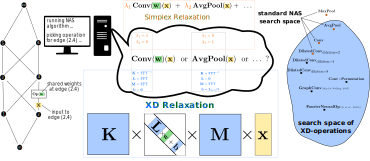
\includegraphics[width=\linewidth]{figures/main/main.pdf}
	\caption{\label{fig:main}
		Diagram of our search space in the single-channel case depicting a NAS method picking an operation to assign to an edge in a backbone network (left).
		Instead of choosing from a discrete search space, we use a relaxation based on the convolution's diagonalization by the discrete Fourier transform in which the DFT matrices are replaced by K-matrices \citep{dao2020kaleidoscope} $\*K$, $\*L$, and $\*M$ (middle);
		these comprise the main architecture parameters of our new search space over Expressive Diagonalization (XD) operations.
		This space contains most operations considered in past NAS research as well as many other important operations in a variety of domains (right).
	}
\end{figure*}

We leverage XD-operations to take critical steps towards a broader NAS that enables the discovery of good design patterns with limited human specification from data in under-explored domains.
To do so we develop a simple procedure which transforms a backbone network into an architecture search space by replacing its operations with XD-operations.
This space is then searched using a simple weight-sharing algorithm that needs only a small amount of tuning to find effective operations.
Finally, we demonstrate the effectiveness of this approach and the need for such a broader class of operations in a series of applications.  
\begin{itemize}[leftmargin=*,topsep=-1pt,noitemsep]\setlength\itemsep{2pt}
	\item We first demonstrate the fragility of NAS operation spaces---and thus the need for XD-operations---with a simple experiment using CIFAR-10.
	While searching over XD-operations and DARTS operations yields comparable performance using the LeNet and ResNet-20 backbones on the original data, models found using XD-operations are 15\% more accurate when the images are permuted.
	In this setting, we even exceed a state-of-the-art NAS algorithm over the DARTS search space by 7\% while using a much smaller model.
	\item We study the problem of solving PDEs, applying XD-operations using a simple convolutional backbone.
	We substantially outperform convolutions and even achieve lower error than the custom-designed, state-of-the-art Fourier Neural Operators (FNOs) of \citet{li2021fno} across three problems with different dimensionalities (Burgers' equation, Darcy Flow, and Navier-Stokes) when comparing to FNOs of the same dimensionality.
	Our method also maintains consistent performance across different resolutions, a major stated advantage of FNOs over previous methods. 
	\item We study four problems in sequence modeling using temporal convolutional networks (TCNs) \cite{bai2018tcn} as backbones.
	By substituting XD-operations we exceed this strong baseline, itself usually better than classical recurrent nets such as LSTMs, on all tasks, including by four perplexity points on word-level Penn Treebank.
\end{itemize}

Code to reproduce these results is available here: \url{https://github.com/nick11roberts/XD}.


%
%\begin{algorithm}[!h]
%	\DontPrintSemicolon
%	\KwIn{input to algorithm}
%	\For{iteration}{
%		do something \tcp*{comment}
%	}
%	\caption{\label{alg:example}
%		algorithm description
%	}
%\end{algorithm}
%
%\begin{table}[!h]
%	\centering
%	\begin{threeparttable}
%		\begin{tabular}{lccccccc}
%			\hline
%			& & \multicolumn{2}{c}{heading}& heading  & heading & heading & heading \\  
%			heading & heading & subheading & subheading & subheading & subheading & subheading & subheading \\
%			\hline
%			section 1$^\ast$ & - & - & - & - & - & - & - \\
%			\hline
%			section 2$^\dagger$ & - & - & - & - & - & - & - \\
%			\hline
%		\end{tabular}
%		\begin{tablenotes}
%			\item[$\ast$] table note 1
%			\item[$\dagger$] table note 2
%		\end{tablenotes}
%		\caption{\label{tab:example}
%			table description
%		}
%	\end{threeparttable}
%\end{table}